\newpage
\section*{Введение}
\addcontentsline{toc}{section}{Введение}

Цель данной главы – анализ применимости новых моделей прогнозирования к задачам государственного управления.

Для достижения указанной цели необходимо решить следующие задачи:
\begin{enumerate}
    \item обзор литературы по теме прогнозирования временных рядов, и в особенности, интеллектуального прогнозирования
    \item выявление сфер применения новых методов прогнозирования, степени их теоретической проработки и практических результатов их использования.    
    \item обзор программных пакетов, позволяющих реализовывать методы нечеткого прогнозирования.
	\item обзор литературы по теме нечеткого прогнозирования социально-экономических процессов.
\end{enumerate}
Работа выполняется по заказу Санкт-Петербургского информационно-аналитического центра.

\newpage
\section{Задачи прогнозирования и интеллектуальный анализ временных рядов}

Количество информации, порождаемой человечеством, непрерывно растет \cite{Gantz2011}. 
В связи с этим все важнее становится умение анализировать данные, извлекать из них знания, чтобы превратить в движущую силу социально-экономического развития. 

Одним из методов анализа данных является прогнозирование. 
Прогнозная аналитика использует методы математического моделирования, искусственного интеллекта и теории игр, 
анализирует текущие и исторические факты для составления предсказаний о будущих событиях. 
Фиксируются связи между разными факторами, на основании их выявления идентифицируются риски и возможности. 
Задача прогнозирования лежит в основе финансового планирования в экономике, управления объемами производства, принятия решений в сфере управления социальными системами.

На сегодняшний день существует множество моделей прогнозирования временных рядов \cite{Chuchueva2012}: регрессионные и авторегрессионные, 
нейросетевые, экспоненциального сглаживания, на базе цепей Маркова, классификационные и др. (Рис. ~\ref{figure:mod_classifier}).
\begin{figure}[bhtp]
    \centering
    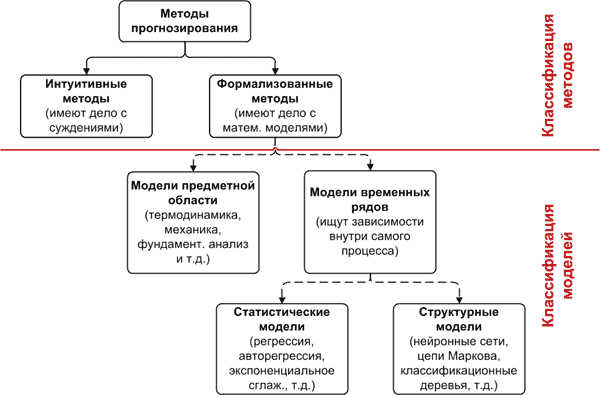
\includegraphics[width=\textwidth, keepaspectratio]{images/mod_classifier.png}
    \caption{классификация моделей и методов прогнозирования \cite{Chuchueva13habr}}
    \label{figure:mod_classifier}
\end{figure}
Прогнозирование в государственном управлении осуществляется посредством разных методов: экстраполяции, факторного прогнозирования, 
модельного прогнозирования, экспертного оценивания. 
Органы государственной власти в последние годы все чаще обращаются к методу экспертного прогнозирования \cite{Gegedush2008}. 
В этом случае эксперт дает прогноз, опираясь на опыт, аналогии, интуицию. 
В то же время интуитивная природа данного метода заставляет при его использовании полагаться лишь на квалификацию и репутацию эксперта, 
тем самым внося дополнительную неопределенность в процесс прогнозирования. 
Существуют исследования, показывающие, что прогнозы экспертов по точности уступают прогнозам на основе моделирования. 
П. Мийл на примере 20 прогнозов из области клинической диагностики \cite{MeehlClinStat} 
и Дж. Сойер на примере 45 прогнозов в социальной сфере \cite{Sawyer1966} демонстрируют тот факт, 
что экспертные оценки ни в одном из перечисленных случаев не были существенно точнее статистических моделей прогнозирования. 
Кроме того, наблюдается нехватка специалистов по работе с данными \cite{Davenport2012}. 
Все это побуждает задуматься о других подходах к анализу данных. 

В последние два десятилетия активно развивается направление прогнозирования, связанное с интеллектуальным анализом временных рядов \cite{Yarushkina2010}. 
Основными целями этого направления являются, во-первых, анализ и моделирование процессов, характеризующихся высокой степенью неопределенности, 
в том числе в областях, слабо подверженных формализации, 
во-вторых, повышение уровня интеллектуальной поддержки современных специалистов, 
и, в-третьих, выявление скрытых закономерностей и извлечение новых знаний из временных рядов. 

\newpage
\section{Сферы применения методов интеллектуального анализа временных рядов}

В основе новых методов анализа временных рядов лежит нечеткая модель временного ряда. 
Теория нечетких множеств была впервые изложена Л. Заде в 1965 г. \cite{zadeh1965fuzzy}. 
В 1973 г. предложена теория нечеткой логики \cite{Zadeh1973}. 
Вскоре после этого теория стала популярна. 
В конце 1980-х гг. это направление стало бурно развиваться в Японии. 
Нечеткое управление стало применяться в промышленности, железнодорожном транспорте и разработке потребительской техники.

\begin{figure}[h]
    \centering
    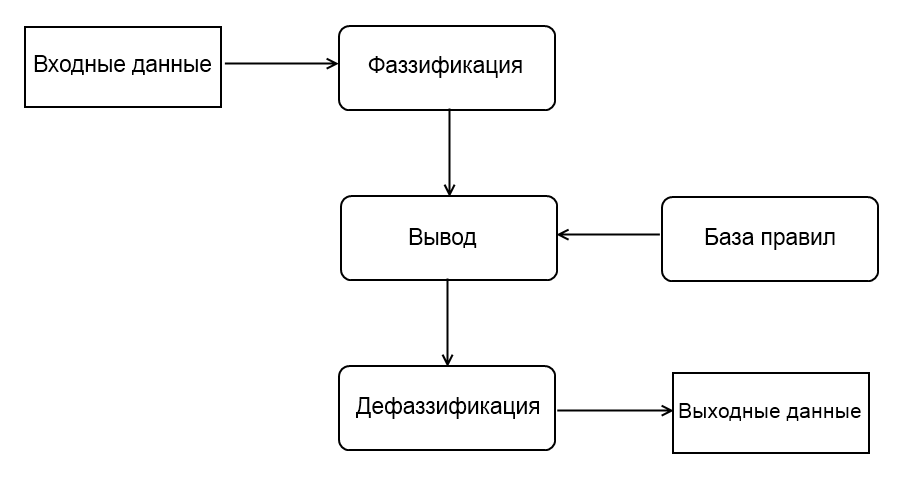
\includegraphics[width=\textwidth, keepaspectratio]{images/fuzzy_engine.png}
    \caption{Система нечеткого вывода}
    \label{figure:fuzzy_engine}
\end{figure}

Основной идеей нечеткой логики является многозначность. 
Высказывание может иметь любое истинностное значение в промежутке от 0 до 1. 
Таким образом, воспроизводится неточность человеческого мышления.

Модели статических и динамических систем, построение, 
использование и анализ которых базируется на положениях теории нечетких множеств и нечеткой логики, называют нечеткими моделями или нечеткими системами. 
Целью нечеткого моделирования сложных явлений является приближенное описание зависимости. 

В основе нечетких продукционных моделей лежит совокупность нечетких правил «ЕСЛИ, ТО», 
описывающих зависимости между нечеткими переменными предметной области, 
композиционное правило вывода и способ вычисления значений нечетких переменных (способ нечеткого вывода).

Модель описания поведения систем на естественном (или близком к естественному) языке,
в виде приближенных рассуждений в теории нечетких множеств и нечеткой логики,
основанная на композиционном правиле вывода, называется системой нечеткого логического вывода.

В систему нечеткого логического вывода входят следующие объекты (рис. ~\ref{figure:fuzzy_engine}):
\begin{enumerate} 
    \item совокупность нечетких продукционных правил (база правил);
    \item блок фаззификации;
    \item блок дефаззификации;
    \item блок вывода.
\end{enumerate}

На основании общей модели, приведенной выше, создаются контроллеры для управления преимущественно техническими объектами.

В начале 1990-х гг. была предложена теория нечетких временных рядов \cite{Song1993}. 
Нечетким временным рядом называют упорядоченную в равноотстоящие моменты времени последовательность наблюдений над некоторым процессом,
состояния которого изменяются во времени, если значение состояния процесса в данный момент времени может быть выражено с помощью нечеткой метки. 
Нечеткая метка может быть сформирована непосредственно экспертом или получена на основе некоторого преобразования исходного временного ряда \cite{Yarushkina2010}. 

В условиях, когда моделируемым процессам присуща высокая степень неопределенности, 
методы прогнозирования на основе нечетких моделей временных рядов позволяют выработать наиболее адекватную оценку будущих изменений в социально-экономических системах.

Ряд исследований \cite{Chen1996,S.Melike2008,Saxena2012}, в которых изучается прогнозирование с помощью моделей нечетких временный рядов, 
демонстрирует положительные результаты. 
Точность прогнозирования улучшается за счет использования генетических алгоритмов для настройки параметров нечетких моделей прогнозирования, 
изменения количества нечетких множеств, используемых для описания временного ряда, использование достаточного числа продукционных правил, 
модификации интервалов, на которые разбивается исходный ряд и др.

В то же время есть примеры неудовлетворительного применения нечеткой логики в прогнозировании временных рядов \cite{Hoekstr2010}. 
Причиной тому неопределенность при создании набора продукционных правил, необходимость адекватного выбора переменных, 
включаемых в модель, сложность построения модели ввиду новизны, малой изученности данной темы и большой вариативности при построении модели.

\newpage
\section{Программные средства интеллектуального прогнозирования}

Для использования прогнозирования в принятии решений целесообразным может
оказаться интеграция этих моделей с экспертной системой или системой поддержки
принятия решений.  В этом случае нужно задуматься о программной реализации
нечетко-логических моделей.  Попробуем рассмотреть существующие библиотеки, в
той или иной мере охватывающие тему нечеткой логики, нечеткого вывода и т.д.

\textit{Fuzzy Logic Toolbox для Matlab}. Хотя данный продукт имеет все
необходимые возможности, для наших задач он не подходит, т.к. функционирует на
собственном языке программирования и зарегистрирован под проприетарной лицензией.

\textit{Fuzzy Logic Toolkit для Octave.} Аналог Fuzzy Logic Toolbox, относящийся
к категории программного обеспечения с открытым исходным кодом. Распространяется
по лицензии GPLv2, ограничивающей его использование в коммерческой деятельности.

\textit{jFuzzyLogic}. Позиционируется как наиболее полная библиотека по нечеткой
логике и стандарт де-факто в исследовательской и прикладной деятельности.
Интересен своей имплементацией языка нечеткого контроля (FCL),
стандартизирующего разработку систем нечеткого вывода. Данный язык соответствует
стандарту IEC 61131-7. Тем не менее, обладает таким недостатком как сложность в
использовании.

\textit{fuzzylite.} Еще одна альтернатива, отличительными чертами которой
являются открытый исходный код, наиболее свободная лицензия, простота в
использовании, наличие различных алгоритмов вывода, лингвистических переменных,
операторов нечеткой логики. Также планируются дополнения в виде новых нечетких
контроллеров, алгоритмов кластеризации и адаптивных нейро-нечетких систем
вывода. Уникальной особенностью является импорт из трёх и экспорт в шесть
различных языков описания нечетких систем (FLL, FLD, FIS, FCL и др.).  Отдельным
преимуществом является доступность библиотеки в исполнении на трех языках
программирования: C++, Java, Python. Кроме того, автором является доктор наук
(PhD) в области искусственного интеллекта Х. Рада-Вилела \cite{RadaVilela2014}.

\textit{frbs} Пакет frbs написан на языке статистического программирования R.
Это позволяет использовать его в тесной интеграции с другими инструментами и
методами R, предназначенными для работы с временными рядами, прогнозированием,
доступа к различным источникам данным, инструментами как классической
математической статистики, так и с более новыми методами машинного обучения.
Пакет разработан группой авторов из Гранадского университета: аспирантов и
докторов наук. Помимо этого, в последней версии frbs добавлена возможность
использовать универсальный язык для описания нечетких моделей frbsPMML,
являющийся диалектом PMML, языка разметки предиктивных моделей. PMML ---
основанный на XML язык, предлагающий стандарт для описания моделей,
сгенерированных алгоритмами дата-майнинга и машинного обучения. Таким образом,
реализована возможность импорта и экспорта нечетких моделей на языке PMML.

\textit{FuzzyEngine, funzy и др.} либо неполны, либо заточены под чисто учебные цели и поэтому непригодны для наших задач. 

\begin{table}[bhtp]
    \caption{Сравнение программного обеспечения, реализующего методы нечеткой
        логики}
	\begin{center}
        \begin{tabular}{ | c | c | c | c |}
			\hline
            Название пакета & Лицензия & Юзабилити & Платформа \\
			\hline
            Fuzzy Logic Toolbox & Проприетарная & Хорошее &
            Win, Linux, Mac\\
			\hline
            Fuzzy Logic Toolkit & Свободная & Хорошее &
            Win, Unix, Unix-like\\
			\hline
            jFuzzyLogic & Свободная & Удовл. &
            Java\\
			\hline
            fuzzylite & Свободная & Отличное &
            Java, C++, Python\\
			\hline
            frbs & Свободная & Хорошее &
            R\\
			\hline
		\end{tabular}		
	\end{center}
    \label{table:soft_comparison}	
\end{table}

По итогам обзора можно выделить fuzzylite и frbs в качестве основных
претендентов к использованию. Однако, в ходе дальнейшего исследования было
обнаружено, что пакет fuzzylite ориентирован преимущественно на программирование
нечетких контроллеров, а не на аналитическую работу с временными рядами. В то
время, как пакет frbs заточен под работу с временными рядами (регрессия) и
категориальными переменными (классификация). Учитывая специфику задачи
прогнозирования временных рядов по социально значимой тематике, целесообразно
выбрать пакет frbs в качестве основного инструмента для прогнозирования с
помощью нечеткой логики.

\newpage
\section{Обзор литературы по нечеткому социальному прогнозированию}

Первые случаи применения теории нечеткой логики связаны с созданием контроллеров для управления техническими системами. Так, в 1987 году в японском городе Сендай была открыта железнодорожная линия, на пассажирских поездах которой были установлены нечеткие системы, регулирующие ускорение, торможение и остановку поезда. С тех пор применение нечетких контроллеров значительно возросло, затрагивая, к примеру, производство бытовой техники (кондиционеры, посудомоечные машины, пылесосы), автомобилестроение (повышение энергоэффективности двигателей), распознавание образов и др.

Однако, перспективы применения нечеткой логики для моделирования и прогнозирования социально-экономических процессов остаются малоизученными. Данный небольшой обзор рассматривает работы по нечеткому прогнозированию с использованием данных государственной статистики. 

В статье  Н. А. Абдуллаевой \cite{Abdullaeva2010} исследуется уровень бедности в Азербайджане в зависимости от доходов населения, коэффициента безработицы, уровня
инфляции и прожиточного минимума, а также дается прогноз
уровня бедности на три года. Для прогноза уровня бедности предлагается нечеткая регрессионная модель. Утверждается превосходство нечеткого регрессионного моделирования перед классическим регрессионным моделированием при прогнозировании уровня бедности, так как оно обеспечивает большую точность результатов. 

Работа М. Г. Мамедовой и З. Г. Джабраиловой \cite{Mamedova2005} 
показывает целесообразность применения нечеткой логики в моделировании демографических аспектов рынка труда на примере задачи прогнозирования численности экономически активного населения. Предложена методика прогнозирования численности экономически активного населения с
использованием модели нечетких временных рядов. Установленный горизонт прогнозирования --- три года. Кроме того, метод применен для долгосрочного прогнозирования (до 2025 года). Проведен сравнительный анализ и интерпретация полученных прогнозных данных для экономически активного, общего и трудоспособного населения, позволившие определить вероятное перспективное состояния рынка труда. 

В статье П. С. Пака и Г. Кима \cite{Pak2005} предлагается основанный на теории нечеткости метод прогнозирования численности и состава населения (пол, возраст, район проживания) на долгосрочный период. На первом этапе представлена нечеткая модель, состоящая из набора правил типа <<если-то>>, для оценки общего роста населения в 402 районах региона Кансай. Антецеденты и консеквенты правил построены с помощью реальных данных, и эти правила составляют нечеткие высказывания и регрессионные модели, соответственно. На втором этапе описан метод для оценки социального роста по полу и возрасту в каждом районе на основе метода нечеткой кластеризации. Метод ориентирован на оценку долгосрочных социоэкономических изменений в миграции населения. Точность результатов предложенной модели сравнивается с традиционной регрессионной моделью, сравнение оказывается в пользу предлагаемой нечеткой модели.   

Исследование А. Сасу \cite{Sasu2010} предлагает методику прогнозирования демографических процессов на основе теории нечетких временных рядов. Своеобразная особенность модели заключается в её способности прогнозировать требуемый показатель, используя неполные, нечеткие входные данные. Автор утверждает возможность установки практически неограниченного горизонта прогнозирования для данной модели.  

Суммируя информацию из рассмотренных источников, заметим некоторые тенденции:
\begin{itemize}
	\item Более высокая точность нечетких моделей в сравнении с классическими моделями для социального прогнозирования.
	\item Широкий диапазон горизонтов прогнозирования: возможность краткосрочного, среднесрочного, долгосрочного прогнозирования.
	\item Разнообразие сценариев применения нечетких моделей для социально-экономических прогнозов.
\end{itemize}
\section{Теорема о нечеткой аппроксимации}

В 1994 году Б. Коско  доказал теорему о нечеткой аппроксимации (Fuzzy Approximation Theorem) \cite{Kosko1994}, согласно которой, любая математическая система может быть аппроксимирована системой на нечеткой логике. Следовательно, с помощью естественно-языковых высказываний <<если-то>>, с последующей их формализацией средствами теории нечетких множеств, можно сколько угодно точно отразить произвольную взаимосвязь <<входы-выход>> без использования сложного аппарата дифференциального и интегрального исчислений, традиционно применяемого в управлении и идентификации. Практические успехи нечеткого управления получили теоретическое обоснование. 

\begin{theorem}[Теорема о нечеткой аппроксимации]
	\label{theorem:FAT}
	Аддитивная нечеткая система  $F$ равномерно аппроксимирует $f: X\rightarrow Y$, если множество $X$ компактно и $f$ непрерывна.
\end{theorem}

\newpage
\section*{Выводы по главе 2}
\addcontentsline{toc}{section}{Выводы по главе 2}

В работе был проведен обзор литературы, описывающей практическое применение нечетких моделей для социально-экономического прогнозирования. Характерна тенденция положительных результатов, улучшения точности в сравнении с классическими методами.

Приведена теорема, доказывающая, что нечеткие системы являются универсальными аппроксиматорами. Данное утверждение позволяет с уверенностью смотреть на будущее применения нечетких моделей.

На основе обзора методов прогнозирования, анализа динамики применения этих методов в прошедшие десятилетия, 
обзора программных библиотек, реализующих принципы нечеткой логики, сделаны следующие выводы:
\begin{enumerate}
    \item Увеличение размерности и доли неопределенности в наблюдаемых данных приводят к необходимости искать новые методы анализа и прогнозирования данных.
    \item Интеллектуальные методы анализа данных дают противоречивые результаты в силу малой изученности и проблемности данной области. Тем не менее, наблюдается положительная тенденция в сторону уточнения моделей.
    \item Существующие свободно распространяемые программные библиотеки позволяют реализовывать системы нечеткого вывода. 
\end{enumerate}

Рассматриваемые нечеткие модели прогнозирования временных рядов, помимо ликвидации неопределенности и возможности работать со слабо формализуемыми входными данными, 
обладают преимуществом простоты для пользователя благодаря использованию продукционной модели знаний. 
Данная модель оперирует правилами, написанными естественным языком, что позволяет пользоваться и совершенствовать её специалисту в предметной области, 
а не только разработчику метода и программной реализации прогнозирования. 
Это положительно сказывается на адекватности прогноза.

Выбранный подход к прогнозированию с использованием методов интеллектуального анализа временных рядов и нечеткой логики имеет потенциал для того, 
чтобы эффективно решить задачу государственного управления и оценки стратегического развития региона. 
Для этого соответствующее программное обеспечение должно быть внедрено в действующие информационно-аналитические системы. 

Дальнейшая работа будет связана с адаптацией какой-либо нечеткой модели 
и её программной реализацией для опытного оценивания возможностей интеллектуального анализа временных рядов.


